\chapter{Probability Test}
\label{chap:probability}

\begin{quotation}
    \textit{I flip the coin in the air. Heads. I flip the coin in the air.
        Tails. I do this, probably hundreds of times, until finally, ten heads
        in a row. Suddenly it hit me. Despite knowing the odds, despite knowing
        that it might take a long time, we still hope, because we know, no
    matter the odds, there is still a chance.}
\end{quotation}

Probability theory finds its application in many fields today ranging from
finance to medicine. It is a powerful tool that allows us to predict the
future, with a certain degree of surity. Probability theory finds its place in
the field of \ac{ML} too. In 1991,
\citeauthor{ref:denker:1991}, \cite{ref:denker:1991} proposed a way to transform
\ac{ANN} outputs to probability distributions . In 1993,
\citeauthor{ref:neal:1993} \cite{ref:neal:1993} developed the first \ac{MCMC}
sampling algorithm for Bayesian \acp{NN}. This shows that probability theory
can be used as a mechanism for learning in \acp{ANN}.

The purpose of this chapter is to provide the necessary background information
needed to understand probability theory as it plays a vital role in the
formulation of the \ac{BHH}.  The chapter is structured as follows:

\begin{itemize}
    \item
    Section~\ref{sec:probability:probability} gives a brief overview of what
    probability is and how it is used.
    
    \item
    Section~\ref{sec:probability:joint_probability} gives a brief overview of
    how probabilities are interpreted for random events that are considered
    jointly.

    \item
    Section~\ref{sec:probability:cond_probability} introduces conditional
    probability. Brief discussions follow on the \textit{frequentist} view
    of conditional probability as well as the \textit{Bayesian} view of
    conditional probability through \textit{Bayes Theorem}.

    \item
    Section~\ref{sec:probability:likelihood} gives a brief overview of the
    concept of likelihood. A brief discussion follow on how likelihood is used
    alongside probability.

    \item
    Section~\ref{sec:probability:probability_distributions} presents relevant
    probability distributions, including the \index{beta
    distribution}\textit{beta} distribution, the \index{dirichlet
    distribution}\textit{dirichlet} distribution, the \index{bernoulli
    distribution}\textit{bernoulli} distribution, the \index{binomial
    distribution}\textit{binomial} distribution, the \index{categorical
    distribution}\textit{categorical} distributions, and the \index{multinomial
    distribution}\textit{multinomial} distribution.

    \item
    Section~\ref{sec:probability:conjugate_priors} presents the conjugate prior
    probability distributions for the \index{bionomial likelihood}binomial
    likelihood as well as the \index{categorical likelihood}\index{multinomial
    likelihood}categorical/multinomial likelihood.

    \item
    Section~\ref{sec:probability:bayesian_stats} presents \textit{Bayesian}
    statistics. It is shown how Bayes' Theorem can be used as an inferencing
    mechanism. Detailed discussions follow on \index{Bayesian
    optimisation}Bayesian optimisation methods such as \index{Bayesian
    inference}\textit{Bayesian inference} and \index{Bayesian analysis}\textit{Bayesian analysis}.

    \item
    Finally, a brief summary of the chapter is given in
    Section~\ref{sec:probability:conclusion}.
\end{itemize}

\section{Probability}
\label{sec:probability:probability}

In everyday conversation, the term \textit{probability} is a measure of one's
belief in the occurrence of a future event \cite{ref:wackerly:2014}.
Consider flipping an unbiased, fair coin. One could consider the probability of
an outcome, whether it is heads or tails, to be a ratio of the possible number
of outcomes. In the case of a coin, the number of outcomes is just two. This
means that one can \textit{believe} that the coin would land with the head-side
up with $1/2$ odds.

Probability can be inferred and confirmed through past events. The support of
these inferred probabilities get stronger as more and more samples of
independent random events, such as flipping of a fair coin, are gathered.  In
the case of flipping a fair coin, the \ac{CLT} shows that the normalised sum of
events tends toward a normal distribution with a mean value of $0.5$ if the
number of events observed $n$ is large (usually $n \geq 30$)
\cite{ref:wackerly:2014}. This shows that the probability of the coin landing
on heads is $50\%$. An illustration of a coin flipping simulation that shows
the central limit theorem on various sample sizes is provided below:

\begin{figure}[ht]
    \centering
    \begin{subfigure}[b]{0.5\textwidth}
        \centering
        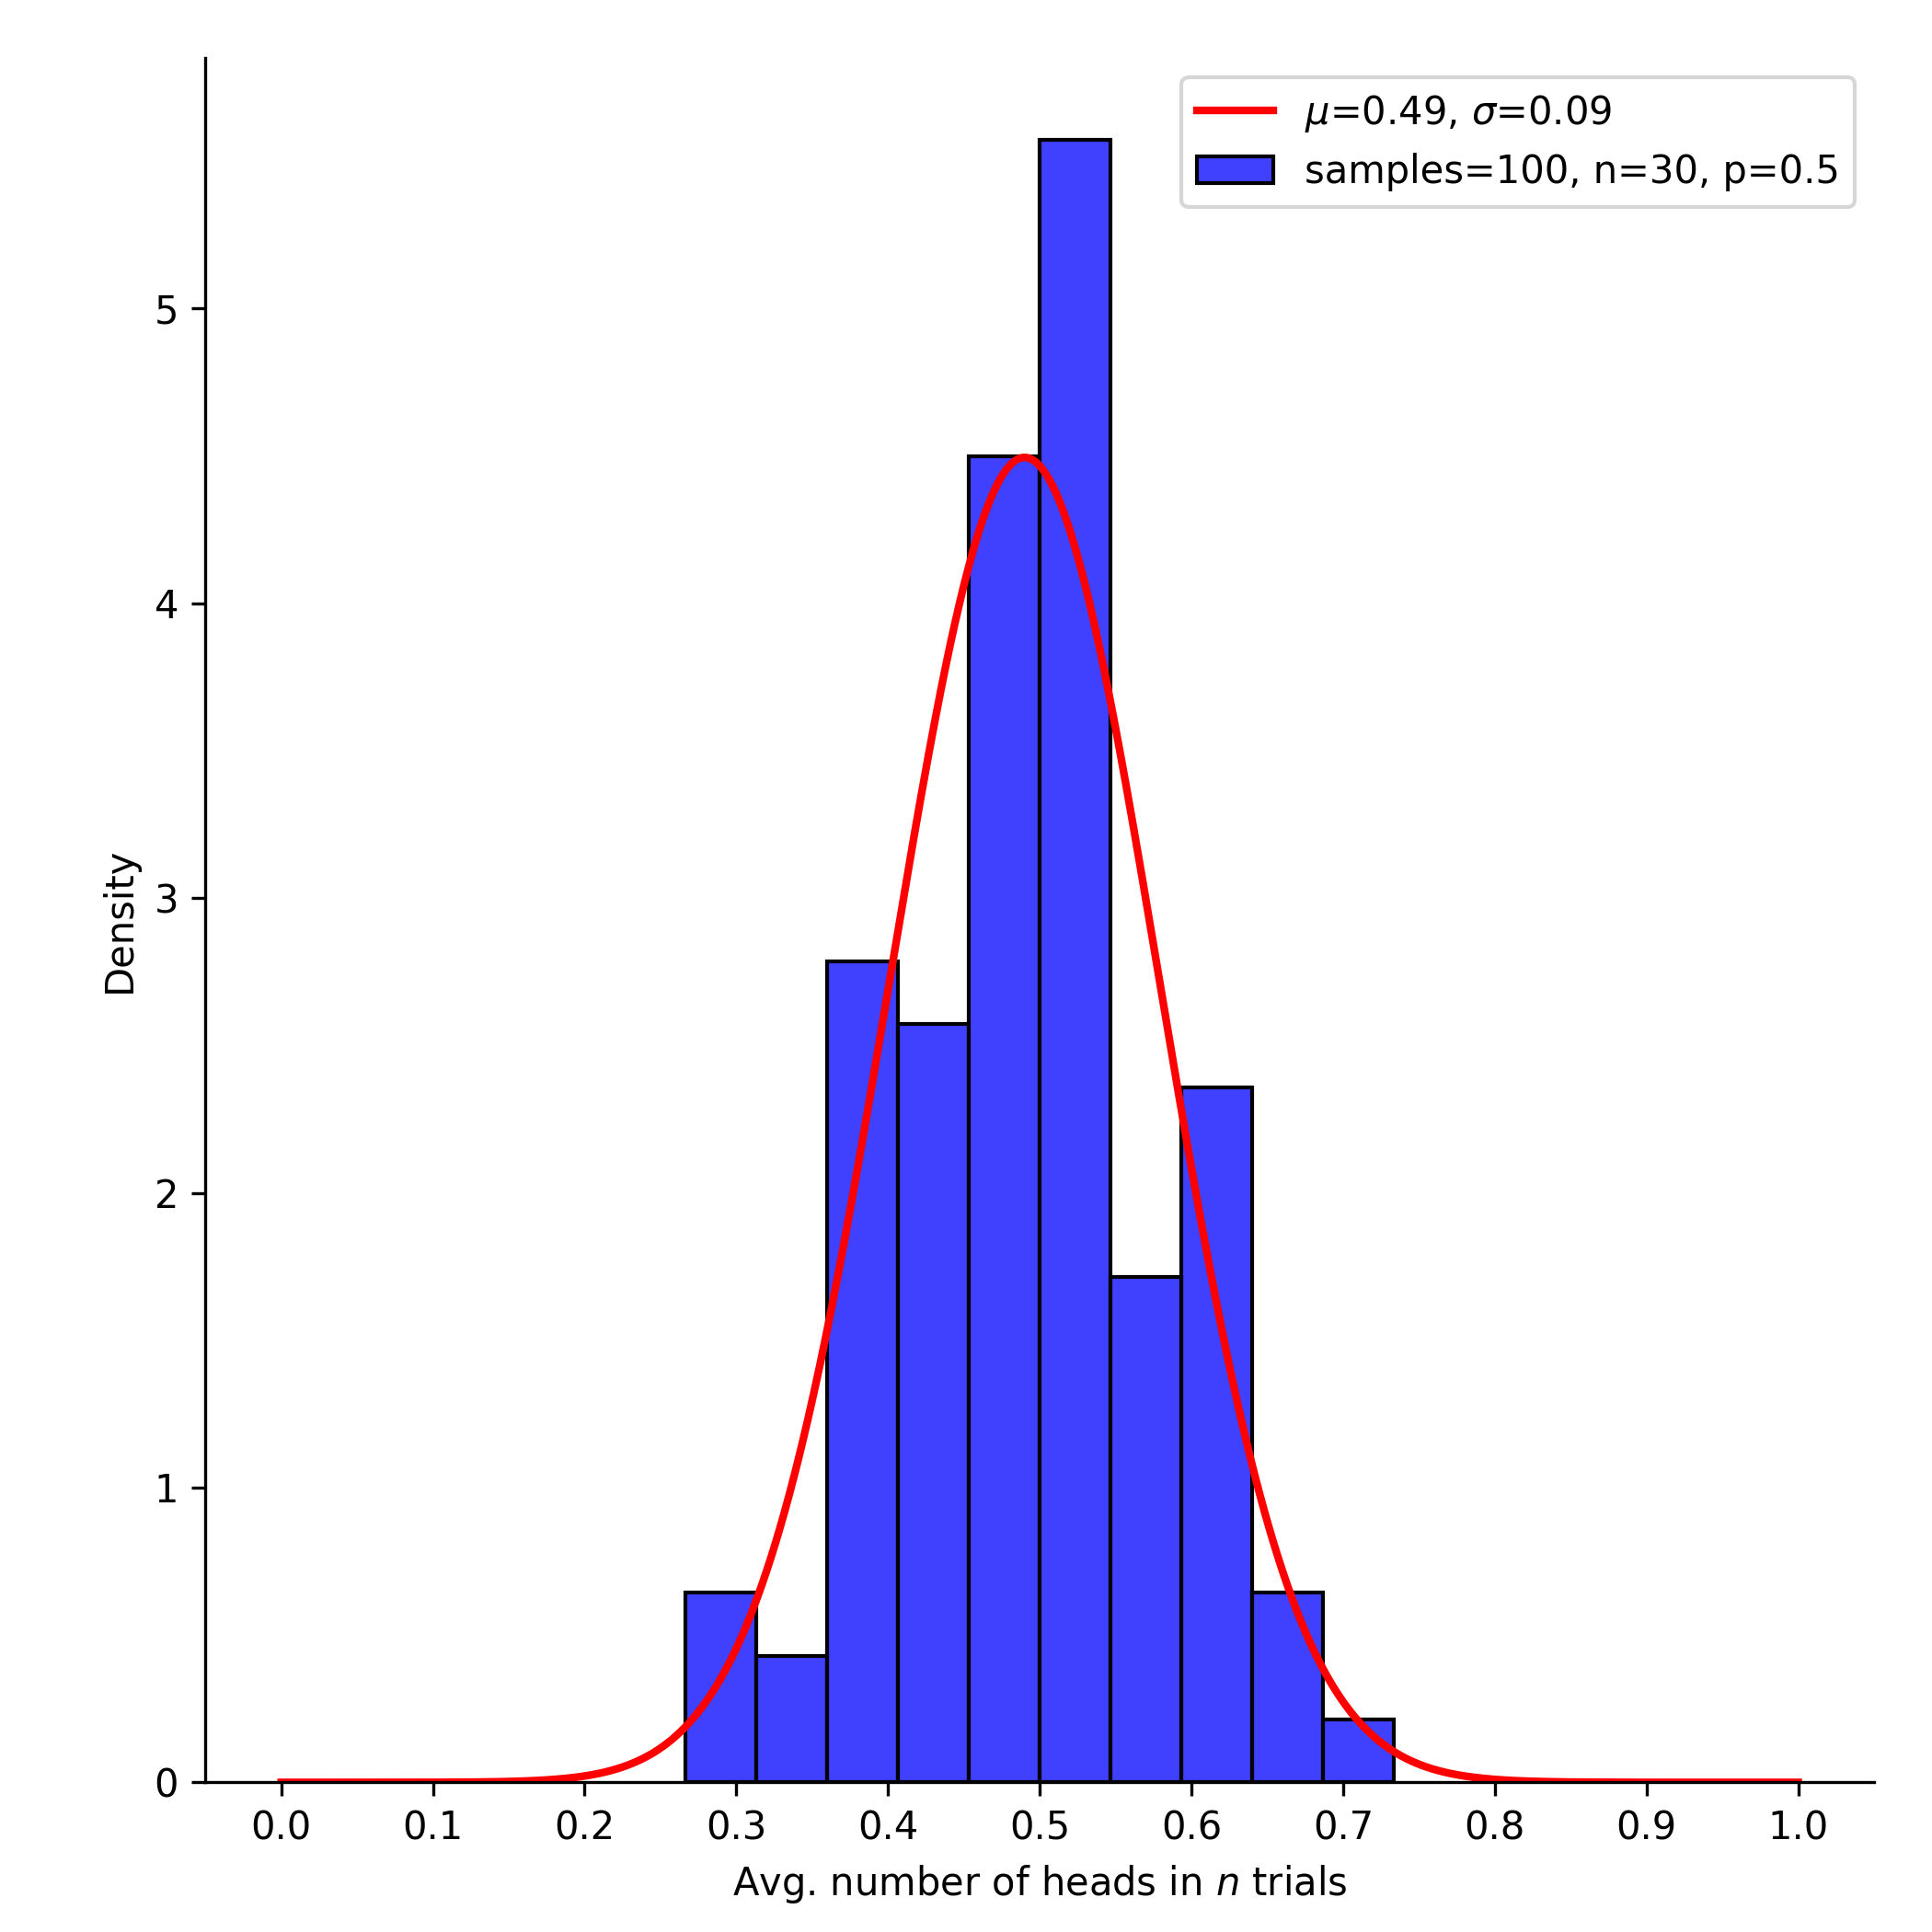
\includegraphics[width=\textwidth]{coin_flip_samples_100.png}
        \caption[Coin flip simulation. Samples=100]{100 samples}
        \label{fig:coin_flip_simulation_samples_100}
    \end{subfigure}
    \hfill
    \begin{subfigure}[b]{0.5\textwidth}
        \centering
        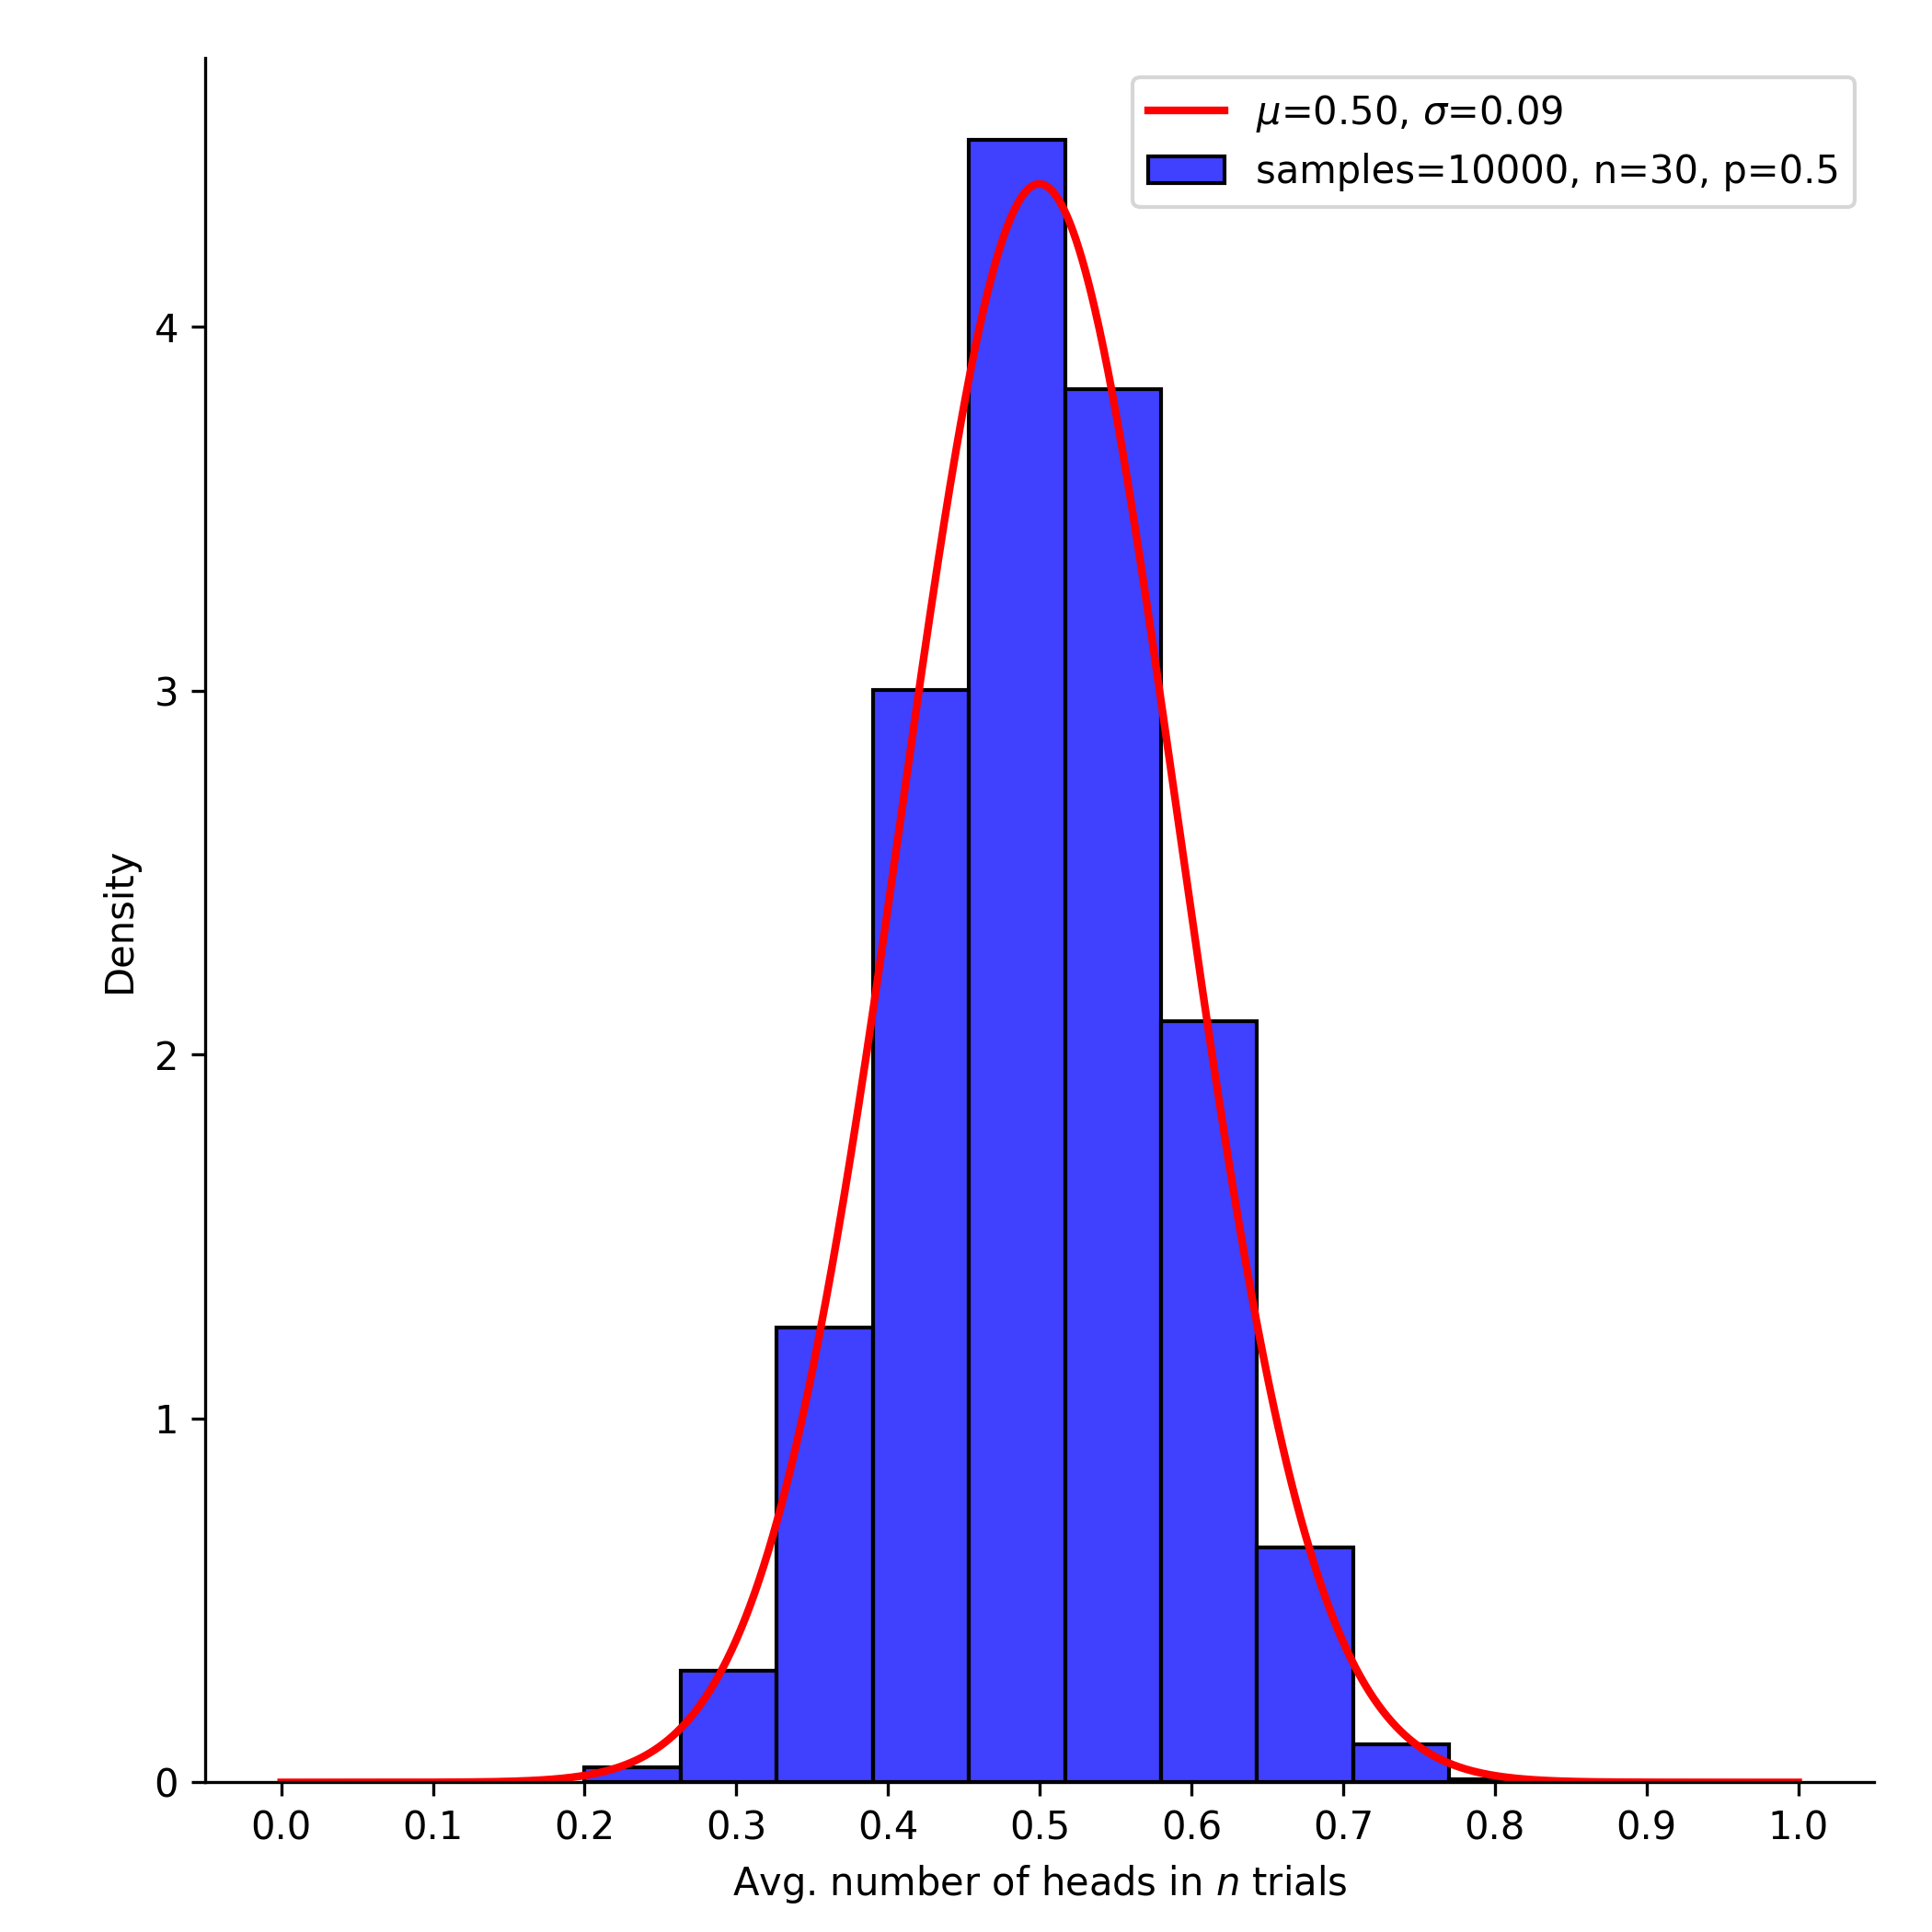
\includegraphics[width=\textwidth]{coin_flip_samples_10000.png}
        \caption[Coin flip simulation. Samples=100]{10000 samples}
        \label{fig:coin_flip_simulation_samples_10000}
    \end{subfigure}
    \caption{An illustration of the \index{central limit theorem}central limit theorem on a coin flip simulation}
    \label{fig:coin_flip_simulation}
\end{figure}








\section{Joint Probability}
\label{sec:probability:joint_probability}












\section{Conditional Probability}
\label{sec:probability:cond_probability}












\subsection{Frequentist}
\label{sec:probability:cond_probability:frequentist}












\subsection{Bayes Theorem}
\label{sec:probability:cond_probability:bayes_theorem}












\section{Likelihood}
\label{sec:probability:likelihood}












\section{Probability Distributions}
\label{sec:probability:probability_distributions}












\subsection{Beta Distribution}
\label{sec:probability:probability_distributions:beta}

The Beta distribution is a family of univariate continuous probability distributions over some $x$, with support on the interval $[0,1]$. It is parametrised by two shape parameters $\alpha > 0, \alpha \in \mathbb{R}$ and $\beta > 0, \beta \in \mathbb{R}$. The Beta distribution is denoted as $Beta(\alpha, \beta)$. The  PDF of the Beta distribution is given below as:

\begin{equation}
P(x | \alpha, \beta) = f_{Beta}(x; \alpha, \beta) = \frac{1}{B(\alpha, \beta)} x^{\alpha - 1} (1 - x)^{\beta - 1}
\end{equation}

where the normalising  constant $B(\alpha, \beta)$ is defined as:

\begin{equation}
B(\alpha, \beta) = \frac{\Gamma(\alpha)\Gamma(\beta)}{\Gamma(\alpha + \beta)}
\end{equation}

and $\Gamma$ is the Gamma function as defined below:

\begin{equation}
\Gamma(n) = ( n - 1)!
\end{equation}

The Gamma function can also be written as:

\begin{equation}
\Gamma(n+1) = n!
\end{equation}

If should be noted that $\alpha$ and $\beta$ determine the shape of the distribution. There exists a special case when $\alpha = \beta$. This is referred to as the symmetric Beta distribution. In the case where $\alpha = \beta = 1$ the distribution is equivalent to the uniform distribution over all points in its support. The Beta distribution for various values of $\alpha$ and $\beta$, including the symmetric version is presented below in figures (???):

INSERT FIGURE HERE.

The expected value of $x$ is given below as:

\begin{equation}
E[x] = \frac{\alpha}{\alpha + \beta}
\end{equation}

Similarly, the expected value of the natural logarithm of $x$ can be calculated as shown below:

\begin{equation}
E[\ln(x)] = \psi({\alpha}) - \psi(\alpha + \beta)
\end{equation}

where $\psi$ is the logarithmic derivative of the Gamma function, called the Digamma function. The Digamma function is defined below as:

\begin{equation}
\psi(n) = \frac{d}{dn}\ln(\Gamma(n)) = \frac{\Gamma'(n)}{\Gamma(n)}
\end{equation}

Finally, the mode of the distribution is given below as:

\begin{equation}
Mo[x] = E[x] - 1 = \frac{\alpha - 1}{\alpha + \beta - 1}
\end{equation}










\subsection{Dirichlet Distribution}
\label{sec:probability:probability_distributions:dirichlet}


The Dirichlet distribution is a family of multivariate continuous probability distributions over some $x$ in $K$ dimensions. The Dirichlet distribution is the multivariate generalization of the Beta distribution and is thus sometimes referred to by its alternative name, the Multivariate Beta Distribution (MBD). The Dirichlet distribution is parametrised by some vector $\alpha = (\alpha_{1}, \dots, \alpha_{K}), \forall_{k=1}^{K} \alpha_{k} > 0, \alpha_{k} \in \mathbb{R}$. $\alpha$ is referred to as the  concentration parameter. The Dirichlet distribution of order $K \geq 2$ with parameters $\alpha$, denoted $Dir(\alpha)$, has a PDF as given below:

\begin{equation}
P(x | \alpha) =  f_{Dir}(x; K, \alpha) = \frac{1}{B(\alpha)}  \prod_{k=1}^{K} x_{k}^{\alpha_{k} - 1}
\end{equation}

where the normalising constant $B(\alpha)$ is defined as:

\begin{equation}
B(\alpha) = \frac{\prod_{k=1}^{K} \Gamma(\alpha_{k})}{\Gamma(\alpha_{0})}
\end{equation}

and $\alpha_{0}$ is defined as:

\begin{equation}
\alpha_{0} = \sum_{k=1}^{K}\alpha_{k}
\end{equation}

Importantly, the set $\{x_{k}\}_{k=1}^{K}$ belongs to the standard $K-1$ probability simplex $S$, meaning that $x_{K} = 1 - \sum_{k=1}^{K-1}x_{k}$ with support $\forall_{k=1}^{K} x \in [0,1]$. Under the simplex $S$, this means that the sum over all values of the vector $x$ must be 1. The simplex can thus be rewritten as $\sum_{k=1}^{K}x_{k} = 1$.

Similar to the Beta distribution, $\alpha$ determines the shape of the distribution in $K$ dimensions and thus, there also exist a special case, referred to as the symmetric distribution when $\forall_{k=1}^{K} \alpha_{k} = c$, where $c$ is some constant. In the case where $c = 1$, the distribution is referred to as a flat distribution and yields the uniform distribution over all points in $S$. The Dirichlet distribution of order $K = 3$, for various values of $\alpha$ , including the symmetric version is presented in figures (???) below:

INSERT FIGURE HERE.


The expected value of $x$ is given below as:

\begin{equation}
E[x_{k}] = \frac{\alpha_{k}}{\alpha_{0}}
\end{equation}

Similarly, the expected value of the natural logarithm of $x_{k}$ can be calculated as follows:

\begin{equation}
E[\ln(x_{k})] = \psi({\alpha_{k}}) - \psi(\alpha_{0})
\end{equation}


where $\psi$ is the Digamma function as defined in Equation (???). Finally, the mode of the distribution is given as:

\begin{equation}
\begin{split}
	Mo[x_{k}] &= E[{x_{k}] -K^{-1}} \\
		&=  \frac{\alpha_{k} - 1}{\alpha_{0} - K}
\end{split}
\end{equation}













\subsection{Bernoulli Distribution}
\label{sec:probability:probability_distributions:bernoulli}

The Bernoulli distribution is a discrete probability distribution over some random variable $x$ that takes the value of $1$ with probability $\theta$ and $0$ with probability $1-\theta$. It is denoted as $Ber(\theta)$ with support $x \in \{0, 1\}$. In probability theory, the Bernoulli distribution is often used to explain the possible outcomes of a single experiment that asks a \textit{yes-no} question such as flipping a coin (ref ???). The outcome of such an experiment is a boolean value. The Bernoulli distribution has a PMF as given below:

\begin{equation}
P(x | \theta) = f_{Ber}(x; \theta) =
	\begin{cases}
		\theta & \text{if}\ x=1 \\
      	1 - \theta & \text{if}\ x=0
	\end{cases}
\end{equation}

The above equation can also be expressed as:

\begin{equation}
f_{Ber}(x; \theta) = \theta^{x}(1-\theta)^{1-x}
\end{equation}

% (See 3rd paragraph: $https://en.wikipedia.org/wiki/Central_limit_theorem$???). 
\todo[inline]{See comment in code}
The mean of the Bernoulli distribution approaches $\theta$ over many samples as
explained in the Central Limit Theorem The expected value of the distribution is thus given as:

\begin{equation}
E[x] = \theta
\end{equation}

while the mode of the distribution is given as:

\begin{equation}
Mo[x_{k}] = 
\begin{cases}
	0 & \text{if}\ \theta < 0.5 \\
    	0,1 & \text{if}\ \theta = 0.5 \\
    	1 & \text{if}\ \theta > 0.5 \\
\end{cases}
\end{equation}




\subsection{Binomial Distribution}
\label{sec:probability:probability_distributions:bin}


The Binomial distribution is a discrete probability distribution over a random variable $x$ taking on a number of successes, in $N$ sequential independent experiments that each ask a \textit{yes-no} question. The probability of a single independent experiment yielding a success is given as $\theta$ and the Binomial distribution is denoted as $Bin(N, \theta)$ with support $x \in \{0, 1, \dots, N\}$.  It should be noted that the Binomial distribution is the extension of the Bernoulli distribution over $N$ independent sequential experiments and thus, each experiment also yields some boolean outcome. When $N=1$, the experiment is referred to as a Bernoulli trial and the distribution is just a Bernoulli distribution and when $N > 1$, the sequence of outcomes is referred to as a Bernoulli process. The PMF of the Binomial distribution is given as follows:

\begin{equation}
    P(x \vert \theta; N) = f_{Bin}(x; N, \theta) = \binom{N}{x} \theta^{x}(1-\theta)^{1-x}
\end{equation}

The mean of the Binomial distribution is just $N\theta$ given the Central Limit Theorem (See paragraph 3 $https://en.wikipedia.org/wiki/Central_limit_theorem$ ???). The expected value of the Binomial distribution is thus given as:

\begin{equation}
E[x] = N\theta
\end{equation}

while the mode of the distribution is given as:

\begin{align}
\begin{split}
Mo[x_{k}] &= E[x] + \theta \\
	&= N\theta  + \theta \\
	&= (N  + 1)\theta
\end{split}
\end{align}



\subsection{Categorical Distribution}
\label{sec:probability:probability_distributions:categorical}

The Categorical distribution is a discrete probability distribution over some random variable $x$, taking on any one of $K$ possible categories. There is no innate underlying ordering to these categories, so for simplicity, each category is assigned a numerical representative value such that $k = (1, \dots, K)$. The probabilities for all outcomes is given by the probability vector $\theta = (\theta_{1}, \dots, \theta_{K})$.  This means that the probability $P(x=k)=\theta_{k}$, with support $x \in \{1, \dots, K\}$. The Categorical distribution, denoted $Cat(\theta)$ is the generalization of the Bernoulli distribution and is sometimes referred to it by its alternative names, the Generalized Bernoulli Distribution (GBD) or the Multinoulli distribution. In probability theory, the Categorical distribution is often used to explain the outcome of a single experiment with more than two possible outcomes such as rolling a die (ref ??). The PMF of the Categorical distribution is given as:

\begin{equation}
P(x | \theta; K) = f_{Cat}(x; K, \theta) = \prod_{k=1}^{K}\theta_{k}^{[x = k]}
\end{equation}

where $[x = k]$ is the Iversion Bracket (ref ???), yielding 1 if $x = k$ and 0 otherwise. From this, one can conclude that:

\begin{equation}
f_{Cat}(x=k; K, \theta) = \theta_{k}
\end{equation}

The random variable $x$ can also be encoded in binary format, yielding a vector $x = (x_{1}, \dots, x_{K})$ of Bernoulli distributions such that the support is $\forall_{k=1}^{K} x_{k} \in \{0, 1\}$. Importantly, if the outcome of the random event is of category $k$, then $x_{k} = 1$ and $\forall_{j=1}^{K} x_{j} = 0, j \neq k$ so that the standard $K-1$ probability simplex $S$ still holds. The PMF of the Categorical distribution can then be rewritten as follows:

\begin{equation}
f_{Cat}(x; K, \theta) = \prod_{k=1}^{K}\theta_{k}^{\mathbbm{1}_{1}(x_{k})}
\end{equation}

where $\mathbbm{1}(x_{k})$ is the Indicator Function, yielding 1 if $x_{k} = 1$ and 0 otherwise.

Since there is no innate order to the underlying categories, the mean of the distribution does not yield any relevant information (ref??). The mode of the distribution is given below as:

\begin{equation}
Mo[x] = \argmax_{k}(\theta_{1}, \dots, \theta_{K})
\end{equation}


\subsection{Multinomial Distribution}
\label{sec:probability:probability_distributions:multinomial}

The Multinomial distribution is a discrete probability distribution over some random variable $x = (x_{1}, \dots\, x_{K})$ that takes on the counts for each occurrence of $K$ possible classes in $N$ independent trials. The probabilities for all possible outcomes in a single trial is given by the probability vector $\theta = (\theta_{1}, \dots, \theta_{K})$. The Multinomial distribution, denoted $Mul(N, K, \theta)$, is thus the generalization of the Binomial distribution to $K$ dimensions. Note that when:

\begin{itemize}
	\item When $K$ is 2 and $N = 1$, the Multinomial distribution is the Bernoulli distribution.
	\item When $K$ is 2 and $N > 1$, the Multinomial distribution is the Binomial distribution.
	\item When $K > 2$ and $N = 1$, the Multinomial distribution is the Categorical distribution.
\end{itemize}
  
The support for the Multinomial is $\forall_{i=1}^{K} x_{k} \in \{1, \dots, N\}, \sum_{k=1}^{K}x_{k} = N$ and the PMF for the Multinomial distribution is given as:

\begin{equation}
P(x | \theta; N; K) = f_{Mul}(x; N, K, \theta) = \frac{N!}{\prod_{k=1}^{K}x_{k}!} \prod_{k=1}^{K}\theta_{k}^{x_{k}}
\end{equation}

Similar to the Categorical distribution, the random variable $x$ can also be encoded in binary format, yielding an $N \times K$ matrix $X$ of Bernoulli distributions. The support is then given as $X \in \{0, 1\}^{N \times K}, \forall_{i=1}^{N}\sum_{k=1}^{K} x_{i,k} = 1$ so that the standard $K-1$ probability simplex $S$ still holds for each trial. The PMF of the Multinomial distribution can then be rewritten as follows:

\begin{equation}
\begin{split}
f_{Mul}(x; N, K, \theta) &= \frac{N!}{\prod_{k=1}(\sum_{i=1}^{N}x_{i, k})!}\prod_{i=1}^{N}\prod_{k=1}^{K}\theta_{k}^{\mathbbm{1}_{1}(x_{i,k})} \\
	&= \frac{N!}{\prod_{k=1}(\sum_{i=1}^{N}x_{i, k})!} \prod_{k=1}^{K}\theta_{k}^{\sum_{i=1}^{N}\mathbbm{1}_{1}(x_{i,k})} \\
	&= \frac{N!}{\prod_{k=1}(\sum_{i=1}^{N}x_{i, k})!} \prod_{k=1}^{K}\theta_{k}^{N_{k}} \\
\end{split}
\end{equation}

where $N_{k}$ is a summary variable denoting the number of times a category $k$ occurs over all trials in $N$. The reason why the Categorical and Multinomial distributions are presented as binary encoded vectors is to simplify the proof of their conjugate priors as will be shown next. This is further supported by the fact that NNs often use binary encoding of feature vectors. The combination of these probabilitic methods and NNs forms the basic of this research dissertation.






\section{Conjugate Priors}
\label{sec:probability:conjugate_priors}












\subsection{Binomial Likelihood}
\label{sec:probability:conjugate_priors:binom_likelihood}

The conjugate prior to a Bernoulli distribution is the Beta distribution
(ref???). This is shown by demonstrating that the posterior distribution has the
same functional form $\mathcal{A}(v)$ as the prior distribution as follows: \\
\textbf{Setup}:

\begin{itemize}
	\item Let $I$ be a number of independent, identical  (iid) random events.
	\item Let $\alpha \in \mathbb{R}, \alpha > 0$ and $\beta \in \mathbb{R}, \beta >0$ be the shape parameters to the Beta distribution.
	\item Let $\theta$ be the probability of a success. With $\theta | \alpha, \beta \sim Beta(\alpha, \beta)$.
	\item $P(\theta)$ is the prior probability distribution with the functional form $\mathcal{A}(v)$.
	\item Let $X = (x_{1}, \dots, x_{I})$ be the outcomes of independent, identical random events, each with boolean outcome. That is $x_{i} | \theta \overset{\text{iid}}{\sim} Ber(\theta)$ and thus $\mathcal{L}(x_{i} \vert \theta)$ is the Bernoulli log likelihood.
	\item Let $\mathcal{D}$ denote all the prior data $X, \alpha, \beta$.
	\item Let $N_{1} = \sum_{i=1}^{I} \mathbbm{1}(x_{i} = 1)$ and $N_{0} = \sum_{i=1}^{I} \mathbbm{1}(x_{i} = 0)$.
	\item  The likelihood of the Bernoulli distribution is:
	
\begin{equation}
\begin{split}
	\mathcal{L}(\mathcal{D}) &=  P(\mathcal{D} | \theta) \\
	&\propto \theta^{N_{1}}(1-\theta)^{N_{0}}
\end{split}
\end{equation}

\end{itemize}

\textbf{Then}:

\begin{itemize}
	\item  By Bayes Theorem, the posterior distribution with given prior data $\mathcal{D}$ is given as:
	
\begin{equation}
\begin{split}
	P(\theta | \mathcal{D}) &= \frac{P(\mathcal{D} | \theta) P(\theta)}{P(\mathcal{D})}
\end{split}
\end{equation}

	\item Since the denominator sums to $1$, one could get rid of the denominator and constants for the Bernoulli likelihood and the Beta prior, by expressing the posterior as proportional to:

\begin{equation}
\begin{split}
		P(\theta | \mathcal{D}) &\propto \left[\theta^{N_{1}}(1-\theta)^{N_{0}}\right] \left[\theta^{\alpha - 1} (1 - \theta)^{\beta - 1}\right] \\
		&\propto \theta^{(N_{1} + \alpha) - 1}(1-\theta)^{(N_{0} + \beta) - 1} \\
		&\propto Beta(N_{1} + \alpha, N_{0} + \beta) 
\end{split}
\end{equation}

\item Yielding a posterior of the same functional form $\mathcal{A}(v)$ as the prior, but with updated prior parameters $\alpha' = N_{1} + \alpha$ and $\beta' = N_{0} + \beta$.

\end{itemize}

This shows that the Beta distribution is the conjugate prior to the Bernoulli likelihood.

Furthermore, it should be noted now that this updating of one's prior beliefs by new evidence as shown above forms the basis for this entire research dissertation. (<<Mention something here about the quote from the master algorithm) >> This is shown in more detail in Chapter (???), however, for now, let us now consider the conjugate prior to the Categorical and Multinomial distributions.











\subsection{Categorical and Multinomial Likelihood}
\label{sec:probability:conjugate_priors:cat_mult_likelihood}

The conjugate prior to a Categorical and Multinomail distribution is the Dirichlet distribution (ref???). Similar to the proof of the conjugate prior for the Bernoulli distribution as shown above, this means that the posterior distribution must have the same functional form $\mathcal{A}(v)$ as the prior distribution. This is shown as follows: \\
\textbf{Setup}:

\begin{itemize}
	\item Let $I$ be a number of independent, identical (iid) random events.
	\item Let $K$ be a number of possible outcomes for each event, with $K \geq 2$.
	\item Let $\alpha = (\alpha_{1}, \dots, \alpha_{K}), \forall_{k=1}^{K} \alpha_{k} \in \mathbb{R}, \alpha_{k} > 0$ be the concentration parameters to the Dirichlet distribution.
	\item Let $\theta = (\theta_{1}, \dots, \theta_{K}), \forall_{k=1}^{K} \theta{k} \in (0,1), \sum_{k}^{K} \theta{k} = 1$ be the probability of each class in $K$ and $\theta$ belongs to the standard $K-1$ probability simplex $S$. With $\theta | \alpha \sim Dir(K, \alpha)$. 
	\item $P(\theta)$ is the prior probability distribution with the functional form $\mathcal{A}(v)$.
	\item Let $X = (x_{1}, \dots, x_{I})$ be the outcomes of independent, identical random events, each with $K$ possible outcomes. That is $x_{i} | \theta \overset{\text{iid}}{\sim} Cat(\theta)$ and thus $\mathcal{L}(x_{i} \vert \theta)$ is the Categorical log likelihood.
	\item Let $\mathcal{D}$ denote all the prior data $X, \alpha$.
	\item Let $N = (N_{1}, \dots, N_{K}), N_{k} = \sum_{i=1}^{I} \mathbbm{1}(x_{i,k} = 1)$, denote the counts for each occurrence of a class $k$.
	\item The likelihood of the Categorical and Multinomial distributions is:
	
\begin{equation}
\begin{split}
	\mathcal{L}(\mathcal{D}) &=  P(\mathcal{D} | \theta) \\
	&\propto \prod_{k=1}^{K} \theta_{k}^{N_{k}}
\end{split}
\end{equation}
\end{itemize}

\textbf{Then}:

\begin{itemize}
	\item  By Bayes Theorem, the posterior distribution with given prior data $\mathcal{D}$ is given as:
	
\begin{equation}
\begin{split}
	P(\theta | \mathcal{D}) &= \frac{P(\mathcal{D} | \theta) P(\theta)}{P(\mathcal{D})}
\end{split}
\end{equation}

	\item Since the denominator sums to $1$, one could get rid of the denominator and constants for the Dirichlet prior, by expressing the posterior as proportional to:

\begin{equation}
\begin{split}
		P(\theta | \mathcal{D}) &\propto \prod_{k=1}^{K} \theta_{k}^{N_{k}} \prod_{k=1}^{K} \theta_{k}^{\alpha_{k} - 1}\\
		&\propto \prod_{k=1}^{K} \theta_{k}^{(N_{k} + \alpha_{k}) - 1} \\
		&\propto Dir(K, N + \alpha) 
\end{split}
\end{equation}

\item Yielding a posterior of the same form $\mathcal{A}(v)$ as the prior, but with updated prior parameters $\alpha' = N + \alpha$.

\end{itemize}

This shows that the Dirichlet distribution is the conjugate prior to the Categorical and Multinomial likelihood.









\section{Bayesian Statistics}
\label{sec:probability:bayesian_stats}












\subsection{Bayesian Inference}
\label{sec:probability:bayesian_stats:bayesian_inference}












\subsection{Bayesian Analysis}
\label{sec:probability:bayesian_stats:bayesian_analysis}












\section{Conclusion}
\label{sec:probability:conclusion}



